\chapter{Discussion}\label{ch:discussion}

This chapter discusses the obtained results and further possible improvements or extensions for the proposed solution.
First, it describes several ways the proposed solution can be improved or extended in section~\ref{sec:implementation}.


\section{Improvements and extensions}\label{sec:improvements}

\subsection{Free space}\label{subsec:free-space}

The extension of the proposed solution is to take a different approach to free space.
\definice{Free space} can be defined as a part of the painting placement solution where the painting is not placed.
For example, free space is important in the FLP problem as there is a need for an aisle between the facilities
through which the material transportation takes place~\cite{scholzExtensionsSTaTSPractical2010}.

In the proposed solution, two main parts influence where the free space is created.
It is (1) the placing heuristic and (2) the evaluation function $\pi$, see eq.~\ref{eq:objective}.
Placing heuristic works locally, i.e., only in the allocated area for the painting, and the evaluation
function, although it might be used to define arbitrary free space shape, is not a constraint but a penalization.
Thus, it does not guarantee that the painting placement solution will create a solution with the desired free space.

One possible approach to guarantee free space is the introduction of dummy paintings.
These dummy paintings can be injected during the slicing tree construction.
The resulting painting placement solution will thus, among the paintings, contain free space occupied by dummy paintings.

An example of dummy painting injection can be seen in figure~\ref{fig:dummy-painting}.
The aisle is created between paintings 1,2, and 3 by adding a vertical cut $V$ to the tree.


\begin{figure}[h!]
    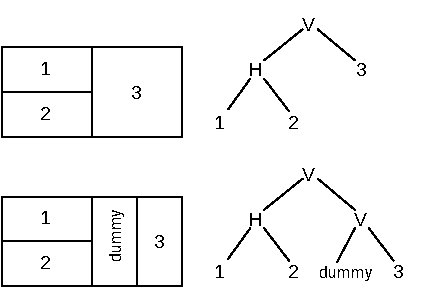
\includegraphics[height=0.33\textheight, center]{dummy_painting}
    \caption[Example of dummy painting injection]{Example of dummy painting injection.}
    \label{fig:dummy-painting}
\end{figure}

\subsection{Non-rectangular layouts}\label{subsec:non-rectangular-layouts}

Another extension to the proposed solution is adding the ability to work with layouts that are not rectangular.
It can be solved using the dummy paintings described in subsection~\ref{subsec:free-space}.
These dummy paintings are as small as possible and placed over the parts of the layout that are not rectangular.
By placing these dummy facilities, the layout becomes rectangular.
A similar approach is used in~\cite{scholzExtensionsSTaTSPractical2010} to modify a slicing tree to solve FLP.

An example of using dummy paintings to work with a non-rectangular layout is in figure~\ref{fig:non-rectangular-layout}.
There are two irregularities in both corners of the layout.
Two dummy paintings are injected into the slicing tree using a dummy painting injection to fill the irregularities.

\begin{figure}[h!]
    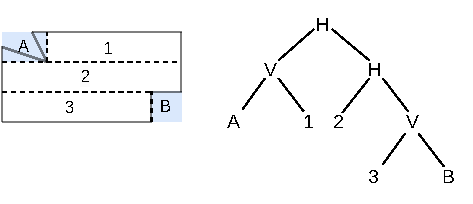
\includegraphics[width=0.8\textwidth, center]{non-rectangular-layout}
    \caption[Example of working with non-rectangular layout]{Example of working with non-rectangular layout. The allocated area is marked using a dotted line.
    Dummy paintings that fill the irregularities in both corners are A and B.}
    \label{fig:non-rectangular-layout}
\end{figure}

\subsection{Non-rectangular paintings}\label{subsec:non-rectangular-paintings}

Not only can the layout be non-rectangular, but also paintings can have a non-rectangular shape.
Thus, another extension is to allow painting shapes that are not rectangular.
This problem can be easily solved by representing a non-rectangular painting
as the smallest possible rectangle to which the painting fits.
By using this approach, the proposed implementation can work with non-rectangular paintings.
One possible drawback is that the painting placement solution might become more sparse,
i.e., containing too much free space.
However, this can be solved using a post-optimization heuristic that tries to reduce a free space
of a painting placement solution.

\subsection{Placing heuristic}\label{subsec:placing-heuristic}

Instead of using the placing heuristic described in~\ref{fig:corner-placing-heuristic}, a different one can be used.
One candidate is a heuristic that, instead of trying to place painting in the corners of the allocated area,
tries to place the painting at all possible placement points, e.g., to place the painting in the middle of the allocated area.
However, using this solution might be computationally expensive.
On the other hand, a heuristic that only tries the bottom-left of the allocated area as a placement point can be much faster but
might not produce good results.

Another approach is calculating suboptimal or optimal placement point inside the allocated area.
Then, move the painting as close as possible to that point.
A similar approach is used in~\cite{goncalvesBiasedRandomkeyGenetic2015} for solving FLP.
They move the facility centroid as close as possible to the calculated unconstrained optimum without leaving the
boundaries where the facility can be placed.

\subsection{Post-optimization}\label{subsec:post-optimization}

One interesting idea is to introduce post-optimization.
This is a process that takes the result, in this case painting placement solution,
and tries to improve it.
For example, if there is not enough free space between a paintings, they can be moved by the post-optimization process.
Another example would be if the goal is to create the most compact layout.
Then, solution can be the compaction operation proposed in~\cite{laiSlicingTreeComplete2001}
which tries to reduce free space between paintings as much as possible.

\subsection{Extension to other problems}\label{subsec:extension-to-other-problems}

This thesis solves the painting placement problem.
The novel genetic approach uses stochastic vector representation with a crossover that adds stochastic vectors together.
This approach can be applied to other optimization problems.
The suitable ones are the ones that optimize some permutation of elements.
For example, elements can be rectangles, and their permutation is used
as an input to a placing heuristic.

One concrete example is 2D-KP problem with rectangular pieces~\cite{bortfeldtGeneticAlgorithmTwodimensional2009},
where the objective is to place as many rectangles in a container as possible,
minimizing unused space.
The solution proposed in this thesis can solve the 2D-KP problem with rectangular pieces by
representing an individual as a stochastic vector that is then decoded
in the same way as the painting sequence random key described in Individual decoding~\ref{subsec:individual-decoding}.
Then, this decoding produces a sequence of rectangles used as an input to BL heuristic~\cite{chazelleBottomnLeftBinPackingHeuristic1983}.
BL heuristic then places all the rectangles inside the container.
After the placing is finished, all rectangles placed outside the container are removed.

\subsection{Future work}\label{subsec:future-work}

There are at least three ideas for the painting placement problem and the proposed implementation that future work might try to address.

\begin{itemize}
    \item Deciding which painting to place.
    \item Multiple walls for painting placement.
    \item Human operator assistance.
\end{itemize}

Deciding which painting to place can happen when the paintings exceed a wall's area.
Thus, some subset of paintings has to be selected and placed.
Also, there can be multiple walls.
Additionally, the walls might have some interactions between them, e.g., placing a painting on the first wall
limits the subset of paintings that can be placed on the second wall.
Lastly, the produced result can be easily visualized.
Thus, it can be used as an input to some human operators that will further modify it.
For example, FLP, see section~\ref{sec:facility-layout-problem}, which creates a layout for multiple facilities.
A human engineer that creates the plan for placing these facilities might use the output of an algorithm as a starting point.
Then, the engineer can modify it by increasing the aisle or changing the position of some facilities.
